\documentclass[a4paper, 10pt]{article}

\usepackage[margin=2cm]{geometry}
\usepackage{hyperref}
\usepackage{graphicx}


\begin{document}

\centerline{\textbf{\LARGE{Hemant Goraksh Ghuge}}}

\vspace{-0.5cm}
\begin{center}
\line(1,0){500}
\end{center}

\begin{center}
\begin{tabular}{ p{10cm} p{10cm} }

B-106, Government Boy's Hostel & +91 91 4594 6493 \\ 
Government College of Engineering and Research & \href{mailto:hemantgghuge@gmail.com}{hemantgghuge@gmail.com} \\      
Avasari(Kh.), Tal$.$ Ambegaon &  \url{in.linkedin.com/in/hemant-ghuge} \\      
Dist$.$ Pune - 412405 & \url{hemantghuge.wordpress.com} \\ 
Maharashtra & 

\end{tabular}
\end{center}

\vspace{-0.5cm}

\begin{figure}[h]
\centering
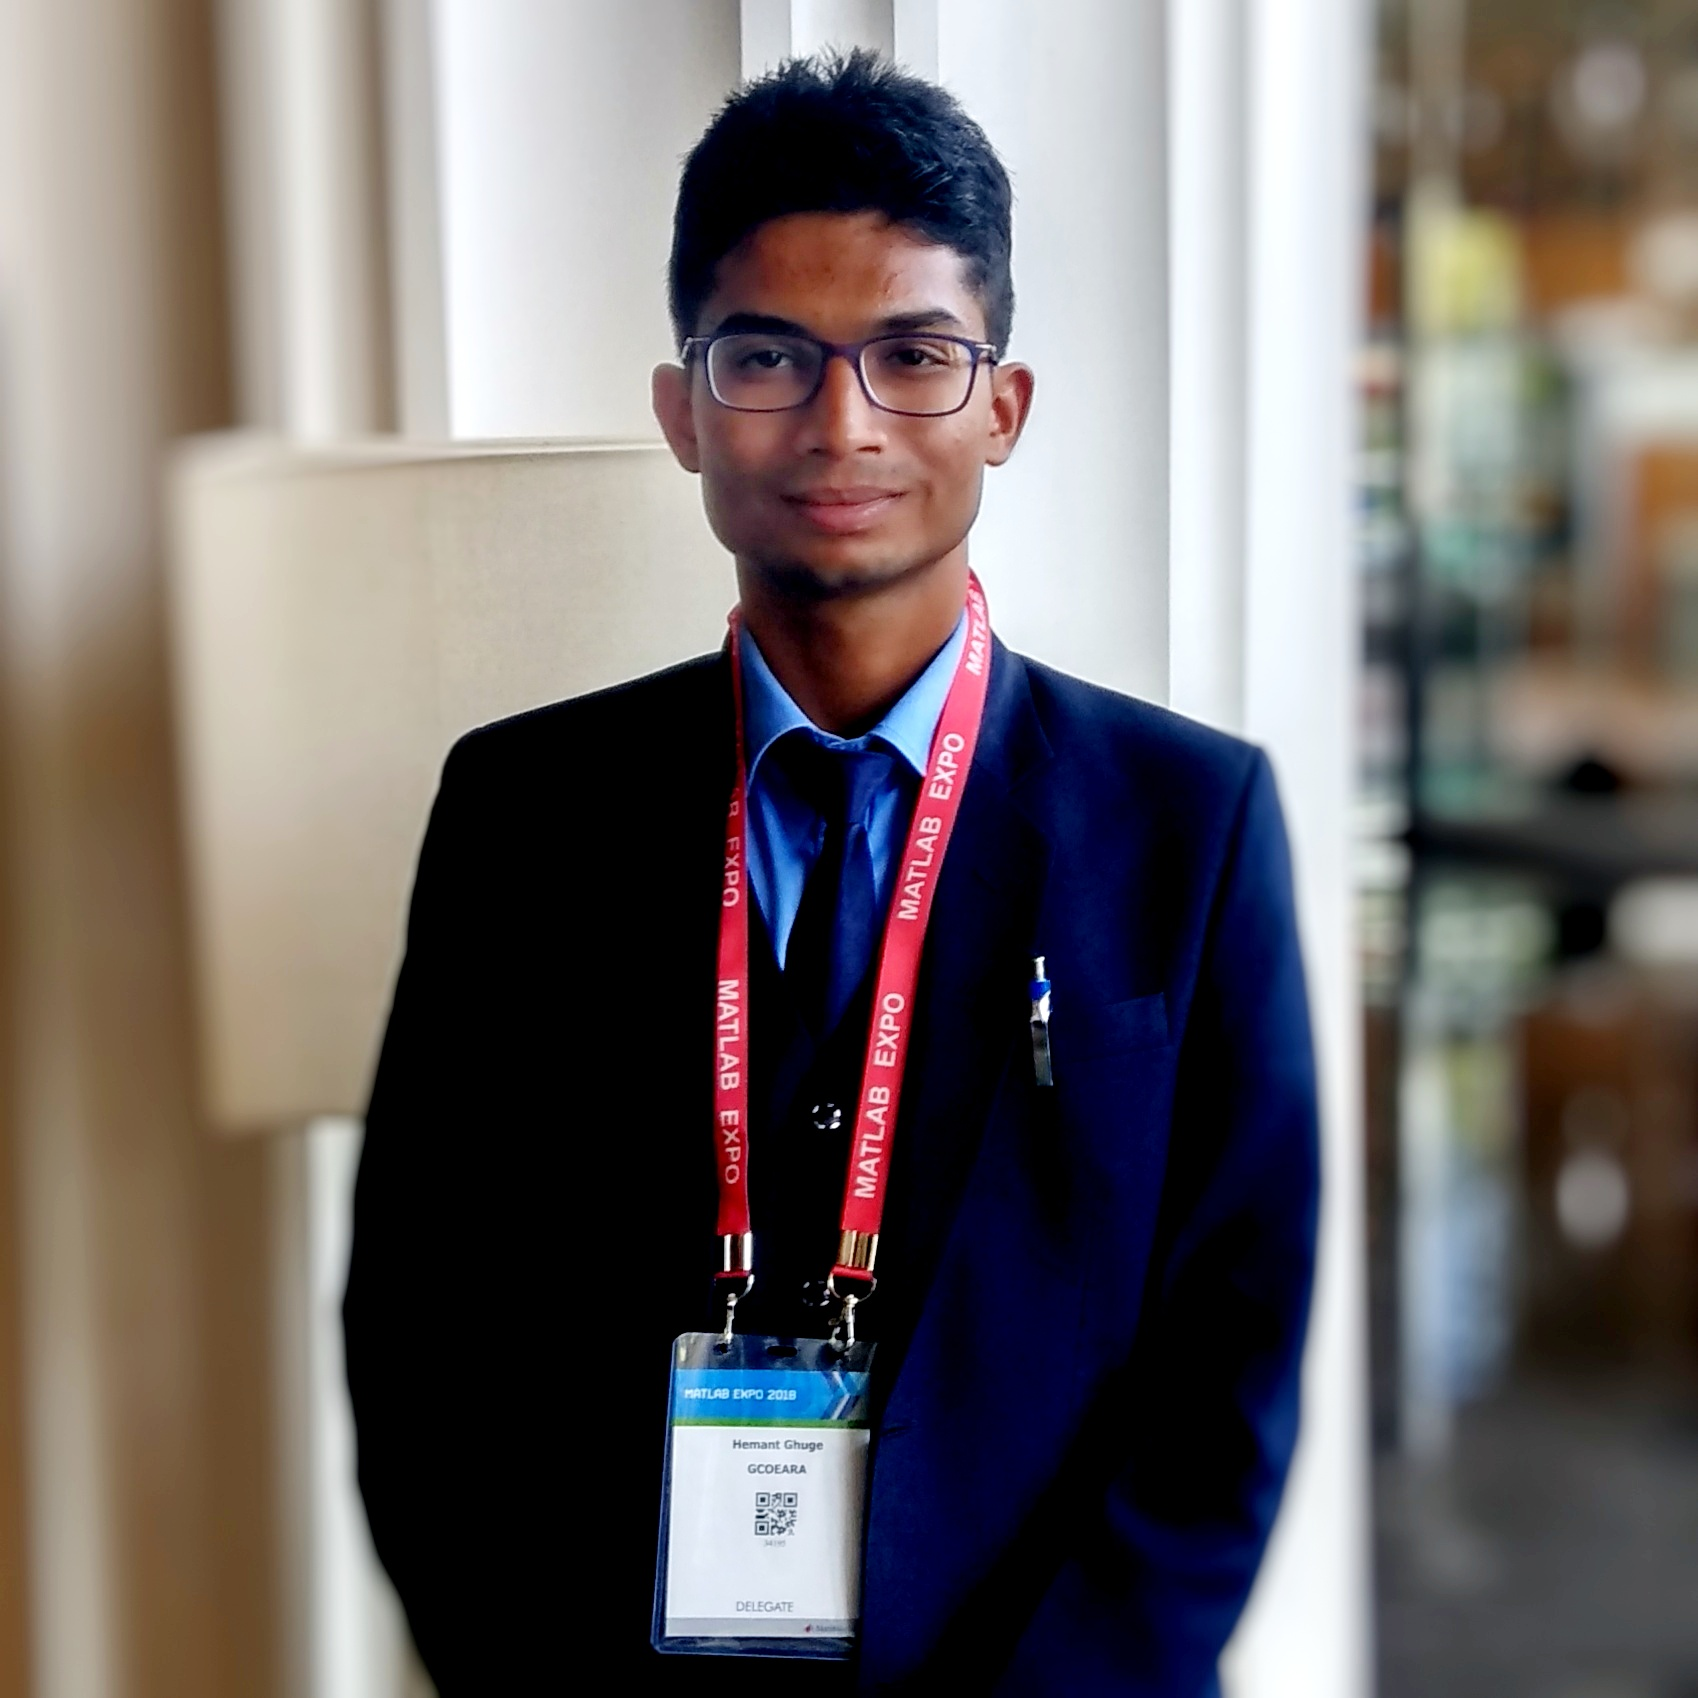
\includegraphics[width=5cm, angle=0]{ResumePhoto.jpg}
\end{figure}

{\textbf{\Large{OBJECTIVE:}}}\\

To pursue a challenging career and be part of a progressive organisation that presents a scope to enhance my knowledge, creativity utilizing my skill toward the development of the organization.\\

{\textbf{\Large{EDUCATION:}}}\\

\vspace{-0.7cm}
\begin{center}
\begin{tabular}{|c|c|c|c|c|}
\hline
\textbf{EXAM} & \textbf{COLLEGE/SCHOOL} & \textbf{BOARD} & \textbf{PASSING YEAR} & \textbf{AGGREGATE}\\ \hline 
B.E & Government College of Engineering and Research &  S.P.P.U & 2020 & 7.76\\ \hline
H.S.C & Army Public School, Mumbai & C.B.S.E & 2016 & 82.8\\ \hline
S.S.C & Army Public School, Mumbai & C.B.S.E & 2014 & 8.8\\ \hline
\end{tabular}
\end{center}

{\textbf{\Large{PROJECTS:}}}
\begin{enumerate}
\item {\textbf{\large{Automated Guided Vehicle (AGV)}}}

Presently I am working on AGV which is Tri-Wheel Omni based vehicle$.$ This AGV can be used in industries to deliver loads.
\item {\textbf{\large{Fire Rescue System (FRS) for High-Rise Building}}}

FRS is a secondary evacuation system used during fire accidents$.$ With this project our team was selected as one of the 21 finalist out of 362 teams in eYantra Idea Competiton held at IIT Bombay and demonstrated our project at National Finals.
\item {\textbf{\large{In-House Mechatronics Kit(33 in 1)}}}

The kit is a custom PCB which covers 33 experiments of SPPU syllabus of 4 branches. It comes under college development projects.
\item {\textbf{\large{ServoEyePi}}}

Raspberry Pi based Computer Vision project using servo motor and pi cam with MATLAB programming. The project was awarded as Innovative Project in Robo-X event - Abinitio 2019 (Technical Event)
\item {\textbf{\large{UltraLine03}}}

Arduino based obstacle avoidance and line following robot which travelled automatic zone of ABU ROBOCON 2018 theme.
\item {\textbf{\large{AlexaPiBhima}}}

Raspberry Pi running amazon's "Alexa voice services"$.$ Python and Bash Scripting were used in this project.
\end{enumerate}

{\textbf{\Large{TRAINING \& INTERNSHIP:}}}
\begin{itemize}
\item MATLAB Onramp training course by MathWorks
\item Deep Learning Onramp training course by MathWorks
\item Drone Making Workhop organised by MindSpark Team (C.O.E.P)
\item First Aid and Life Saving Course conducted under the aegis of Headquarters Southern Command (Medical)
\item Planning to do internship in this summer vacation.\\
\end{itemize}

{\textbf{\Large{RESEARCH PUBLICATIONS:}}}
\begin{enumerate}
\item FRS - Journal Paper - Yet to publish.
\item Automated Guided Vehicle - Conference Paper - Yet to publish. \\
\end{enumerate}

{\textbf{\Large{TECHNICAL SKILLS:}}}
\begin{itemize}
\item MATLAB
\item Simulink
\item C \& Python
\item Raspberry Pi
\item Arduino
\item IoT
\item Bash Script
\item Ubuntu
\item Vim Text Editor
\item Computer Vision
\item Deep Learning \\
\end{itemize}

{\textbf{\Large{SOFT SKILLS:}}}
\begin{enumerate}
\item Communication
\item Multi-tasking
\item Adaptability
\item Team Work
\item Leadership
\item Public Speaking
\item Committed
\item Negotiator \\
\end{enumerate}

{\textbf{\Large{EXTRA-CURRICULAR ACTIVITIES:}}}
\begin{itemize}
\item \textbf{Senior Team Member at Robotics Research Lab, GCOEARA}

Presently participating in National Robotic Contest Robocon 2019$.$ Our team was AIR 2nd (League Table) in National Robotic Contest Robocon 2018.
\item \textbf{Senior Manager at eLSI'19}

We the senior members of eLSI lab work for developing technical skills among other members.
\item \textbf{State Level Football Goalkeeper and Athlete}

Presently I am goal-keeper of Junnar Taluka Football Club (JTFC)$.$ Our team awarded as 2nd Runner-up in 7 a side football championship trophy 2018$.$ Participated 3 times in CBSE Cluster Football as well as Athletic Meet$.$ I was the Sports Captain of Army Public School, Mumbai. 
\item \textbf{Typing Speed 35wpm}

I have too craze in keyboard typing$.$ This craziness made me the winner of typing event at GPA.
\item \textbf{Rubik's Cube Solver}

Solving Rubik's Cube is one of my hobbies$.$ This hobby helped me in securing 2nd place in Rubik's Cube event at GPA.
\item \textbf{Blood Donor}

I have donated my blood three times till now.\\
\end{itemize}

{\textbf{\Large{CO-CURRICULAR ACTIVITIES:}}}
\begin{enumerate}
\item \textbf{SAAGA 2K18}

Member of Student Alumni Association of GCOEARA.
\item \textbf{Workshop}

I have conducted and organised many workshop in college on MATLAB, and Raspberry Pi. Each time we get great feedback from participant.
\item \textbf{Abinito (Technical Event)}

Department Head - Abinitio 2018-19.\\
Sub-Coordinator of Line Tracing Event - Abinitio 2017-18. 
\item \textbf{Resonance (Cultural Event)} 

Branch Theme Winner - Resonance 2017. \\
Street-play event Winner - Resonance 2017.
\item \textbf{Combat (Sports Event)}

Football Competition Winner - Combat 2017. \\
\end{enumerate}

{\textbf{\Large{PERSONAL DETAILS:}}}\\

\begin{tabular}{ p{3cm} p{7cm} }
Father's Name: & Hav$.$ Goraksh Karbhari Ghuge(Retd.) \\ 
Mother's Name: & Aruna Goraksh Ghuge\\      
Sex: & Male \\      
Date of Birth: & January 30, 1999\\ 
Nationality: & Indian \\
Marital Status: & Single \\ 
\\
\end{tabular}

{\textbf{\Large{REFERENCES}}}\\

\begin{tabular}{ p{5cm} p{5.5cm} p{5.5cm} }
Dr$.$ Veer Alakshendra & Dr$.$ Avinash Pant (Principal) & Dr$.$ Manoj Nagmode\\ 
Technical Evangelist & Govt$.$ College of Engg$.$ \& Research & Head, Department of E\&TC \\      
MathWorks & Former Vice Chairman at A.I.C.T.E & Govt$.$ College of Engg$.$ \& Research \\      
8446985971 & 9958411661 & 9226771488 \\ 
Veer.Alakshendra@mathworks.in & pantavinash@hotmail.com & manoj.nagmode@gmail.com \\
\\
\end{tabular}

{\textbf{\Large{DECLARATION}}}\\

\centerline{I hereby declare that the above written particulars are true to the best of my knowlege and belief.}


\end{document}